% Specifies the document class. '10pt' sets the font size.
\documentclass[10pt]{article}

% --- PACKAGE IMPORTS ---
\usepackage{amsmath}        % For advanced math typesetting
\usepackage{amssymb}        % For additional math symbols
\usepackage{graphicx}       % To include images
\usepackage[margin=1in]{geometry} % To set page margins
\usepackage{hyperref}       % For clickable links (URLs, references)
\usepackage{authblk}        % For author affiliations
\usepackage{enumitem}       % For customized lists
\usepackage{algorithm}      % For algorithm environment
\usepackage{algpseudocode}  % For pseudocode
\usepackage{booktabs}       % For nicer tables
\usepackage{tabularx}       % For tables that span a specific width
\usepackage{cite}           % For improved citation handling

\setlength{\columnsep}{20pt} 
% Default is 10pt. Try 15pt, 20pt, or 25pt.

\hypersetup{
    colorlinks=true,
    linkcolor=blue,
    citecolor=blue,
    urlcolor=blue,
    pdftitle={Tactical Trend Trader},
    pdfauthor={Trisagion Developers}
}

\twocolumn

% --- DOCUMENT METADATA ---
\title{%
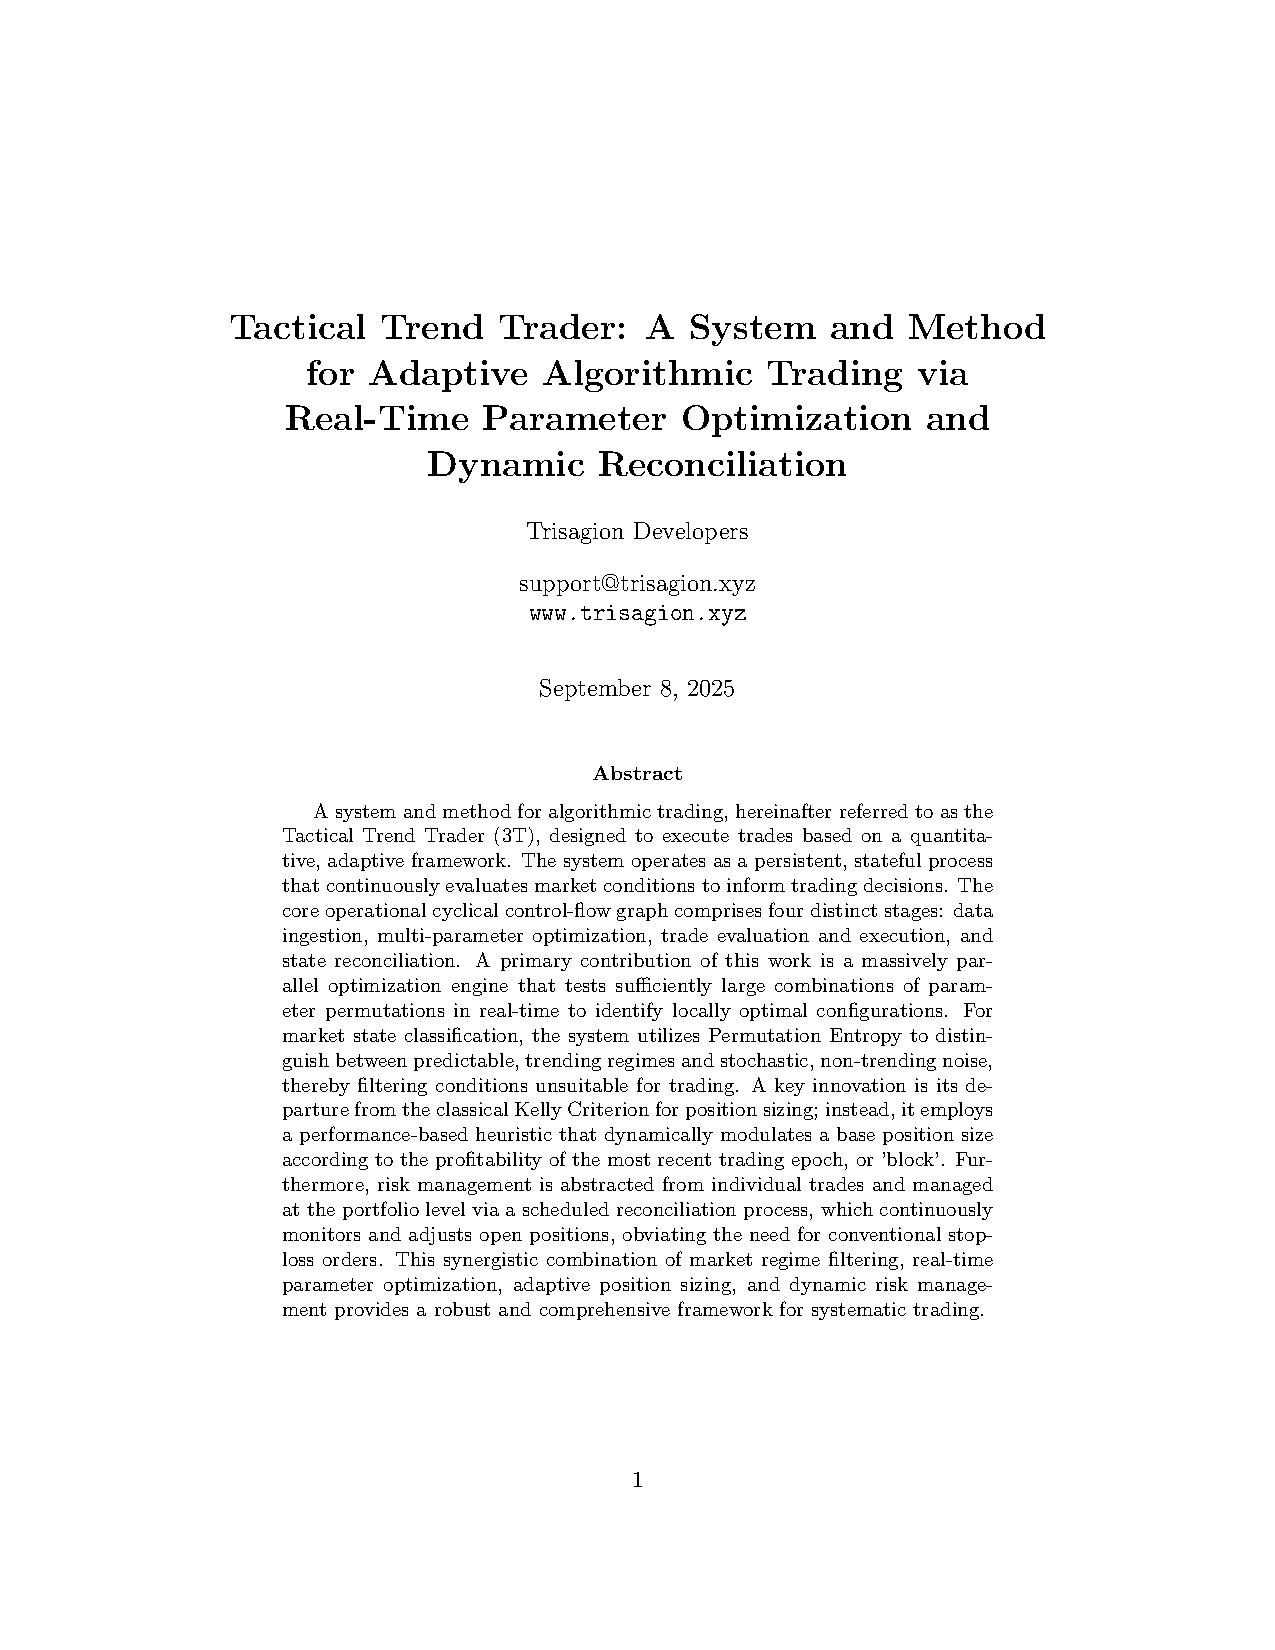
\includegraphics[width=2.5cm]{TTT.pdf}

\textbf{Tactical Trend Trader: A System and Method for Adaptive Algorithmic Trading via Real-Time Parameter Optimization and Dynamic Reconciliation}}
\author{Trisagion Developers \\
        \href{mailto:support@trisagion.xyz}{support@trisagion.xyz} \\
        \url{www.trisagion.xyz}}
\date{\today}

% --- BEGIN DOCUMENT ---
\begin{document}

\maketitle

% --- ABSTRACT ---
\begin{abstract}
A system and method for algorithmic trading, hereinafter referred to as the Tactical Trend Trader (3T), is presented, designed to execute trades based on a quantitative, adaptive framework. The system operates as a persistent, stateful process that continuously evaluates market conditions to inform trading decisions. The core operational cyclical control-flow graph comprises four distinct stages: data ingestion, multi-parameter optimization, trade evaluation and execution, and state reconciliation. A primary contribution of this work is a massively parallel optimization engine that tests sufficiently large combinations of parameter permutations in real-time to identify locally optimal configurations. This architecture is a direct response to the documented limitations of conventional predictive models in non-stationary markets, favoring continuous, exploratory adaptation over retrospective prediction. For market state classification, the system utilizes Permutation Entropy to distinguish between predictable, trending regimes and stochastic, non-trending noise. A key innovation is its departure from the classical Kelly Criterion for position sizing; instead, it employs a performance-based heuristic that dynamically modulates a base position size according to recent profitability. Furthermore, risk management is abstracted from individual trades and managed at the portfolio level via a scheduled reconciliation process, obviating the need for conventional stop-loss orders. This synergistic combination provides a robust framework for systematic trading that addresses the fundamental challenge of adaptation lag inherent in history-bound models.
\end{abstract}

% --- INTRODUCTION ---
\section{Introduction}
The domain of algorithmic trading is characterized by a persistent challenge: developing systems that can adapt to non-stationary and often chaotic financial markets \cite{ref:nonstationarity}. Many conventional systems rely on statically configured parameters, rendering them brittle and susceptible to performance degradation as market dynamics shift. Even sophisticated systems that employ periodic model retraining can fail when confronted with sudden regime shifts, structural breaks, or rare black-swan events.

The Tactical Trend Trader (3T) is a computer-implemented system engineered to address these limitations by integrating real-time adaptability into its core architecture. It is designed to optimize performance by leveraging statistical analysis for market regime detection and a novel set of heuristics for risk and position management.

The current architecture of the 3T is the result of a deliberate evolution away from a more conventional, but ultimately less effective, machine learning paradigm. Early system development focused on a regression-based approach using a sophisticated \textbf{bootstrap-aggregated ensemble} of heterogeneous learners. This ensemble included a Multi-layer Perceptron (MLP), several gradient-boosted tree models (LightGBM, CatBoost, XGBoost), a Random Forest, and a k-Nearest Neighbours classifier \cite{ref:bagging, ref:xgboost, ref:lightgbm, ref:catboost} provided by AutoGluon\cite{ref:autogluon}. This predictive model was re-trained hourly on all accumulated historical observations of the unbiased continuous evaluations with the goal of forecasting the expected profit and loss of potential portfolio positions. During inference, a trade would only be executed against live risk if the predictor scored positively.

However, over a period of several months of study, this predictive approach consistently underperformed. The core issue identified was that models trained on historical data are fundamentally retrospective. Their learned mappings from market features to expected outcomes become stale in the face of new market dynamics, creating a performance-costly "adaptation lag" that persists even after incorporating changes in the next model retrain. The pivotal insight from this empirical investigation was that randomized, out-of-sample feature values were consistently superior to the carefully trained tabular predictors. This finding supports a central thesis: for highly unpredictable environments, \textbf{online stochastic exploration is more effective than classic supervised learning}. Consequently, the machine learning aspect was removed entirely in favor of the current paradigm.

The 3T system now operates in a continuous loop, analyzing market data to first identify predictable, trending environments and then deploying capital with a position size dynamically calibrated to recent system performance. This paper details the mathematical framework, system architecture, and unique operational logic of the 3T. The primary contributions of this method are:

\subsection{A Real-Time Optimization Engine} 

A mechanism that continuously stress-tests a large number of parameter permutations against live market data. This engine is the direct, successful replacement for the abandoned machine learning ensemble. This optimization includes both momentum-following ("breakout")\cite{lefevre1923} and mean-reverting ("swing")\cite{taylor1950} entry strategies simultaneously, allowing for greater tactical flexibility.

\subsection{A Hybrid Risk Management Model}

A novel heuristic for position sizing based on recent performance, coupled with a dynamic, reconciliation-based approach to position control that replaces static, per-trade stop-losses.

% --- RELATED WORK ---
\section{Related Work}
The 3T's architecture is informed by established practices in quantitative finance but represents a novel synthesis that prioritizes real-time adaptation. This section surveys the two competing paradigms—ensemble-based prediction and stochastic optimization—that were empirically tested during the system's development.

\subsection{Ensemble Methods in Financial Prediction}
Ensemble methods, such as bootstrap aggregating (bagging) \cite{ref:bagging} and gradient-boosted trees \cite{ref:xgboost, ref:lightgbm, ref:catboost}, have become standard tools for modeling tabular financial data. Their ability to reduce variance and capture complex, non-linear interactions makes them attractive for tasks like predicting risk-adjusted returns \cite{ref:ensemble_finance}. To combat the non-stationarity of financial time series, online learning and incremental model updating schemes are often employed \cite{ref:online_learning}.

Despite their power, these methods share a fundamental limitation: they rely on a "past-to-present" update rule. A model's knowledge is exclusively derived from historical data. Consequently, they inherit an intrinsic "adaptation lag," rendering them vulnerable to sudden regime shifts where past patterns no longer hold predictive power.

\subsection{Stochastic Optimization in Finance}
An alternative paradigm is stochastic optimization, which includes methods such as simulated annealing \cite{ref:annealing}, evolutionary strategies \cite{ref:evolution}, and random search \cite{ref:random_search}. The primary strength of these techniques lies in their ability to explore a broad search space without being confined to a deterministic gradient or patterns learned from historical data. In finance, they are commonly applied to offline tasks, such as portfolio construction or the hyper-parameter tuning of other models.

\subsection{The 3T's Position: Online Stochastic Policy Generation}
The 3T system's core innovation is to take the principles of stochastic optimization and apply them not as an offline tuning process, but as the central, online, real-time decision-making mechanism. The system's Parameter Optimization Engine functions as a \textbf{continuous stochastic policy generator}. This approach directly addresses the adaptation lag of ensemble methods by continuously testing new parameter sets against live market data, making it a more suitable paradigm for highly dynamic and unpredictable markets. The fundamental differences between these two approaches are summarized in Table~\ref{tab:paradigms}.

\begin{table*}[t]
\small
\centering
\caption{Paradigmatic Comparison of Trading System Approaches.}
\label{tab:paradigms}
\begin{tabularx}{\textwidth}{@{} l >{\raggedright\arraybackslash}X >{\raggedright\arraybackslash}X @{}}
\toprule
\textbf{Feature} & \textbf{Tabular Predictor (Ensemble)} & \textbf{Stochastic Engine (3T)} \\
\midrule
\textbf{Core Task} & Prediction of future Profit \& Loss based on learned patterns. & Adaptation of system parameters to maximize immediate profitability. \\
\textbf{Data Reliance} & Retrospective: Trained exclusively on historical data. & Prospective: Tested continuously on live, real-time data. \\
\textbf{Adaptation Mechanism} & Periodic Batch Retraining (e.g., hourly) on accumulated data. & Continuous Real-Time Perturbation and evaluation of parameters. \\
\textbf{Adaptation Latency} & High (minutes to hours). The model is stale between retraining intervals. & Near-Zero. Adaptation occurs at the frequency of the decision epoch. \\
\textbf{Primary Failure Mode} & Stale mapping during regime shifts, leading to poor decisions based on outdated patterns. & Inefficient exploration if the perturbation variance is poorly tuned. \\
\bottomrule
\end{tabularx}
\end{table*}

% --- SYSTEM ARCHITECTURE ---
\section{System Architecture}
The 3T system is a modular architecture comprising four main components: a Data Ingestion Module, a Parameter Optimization Engine, a Trade Evaluation and Execution Engine, and a State Reconciliation Module. This separation of concerns ensures robustness and scalability.

\subsection{Data Ingestion Module}
This module serves as the sensory input for the entire system, acquiring market data from two primary sources:
\begin{itemize}
    \item \textbf{Real-time Websocket Stream:} Provides low-latency access to immediate price updates (tick data), crucial for the Parameter Optimization Engine.
    \item \textbf{Historical API Endpoint:} Fetches historical Open/High/Low/Close (OHLC) data, providing aggregated into one-minute volatility bars. This provides the necessary historical context for macro-level analysis like Permutation Entropy calculation.
\end{itemize}

\subsection{Parameter Optimization Engine}
This engine operates as a continuous, massively parallel simulation layer that runs concurrently with the live trading system. Its purpose is to find the most profitable set of parameters for the core trading algorithm in the current market environment strictly as a function of out-of-sample performance.

Technically, the engine functions as a stochastic decision engine. At each decision epoch $t$, it generates a candidate policy $\boldsymbol{\theta}_t$ by applying a perturbation vector $\boldsymbol{\epsilon}_t$, drawn from a Gaussian distribution $\mathcal{N}(\mathbf{0},\sigma^2\mathbf{I})$, to a set of base parameters $\boldsymbol{\theta}^{\text{base}}$:
$$\boldsymbol{\theta}_t = \boldsymbol{\theta}^{\text{base}} + \boldsymbol{\epsilon}_t$$
This perturbed policy is then evaluated in a virtual simulation against live market data. The engine employs an \textbf{accept-if-profitable} hill-climbing rule: if the simulated profit-and-loss of the candidate policy is positive, its parameters are adopted for the next evaluation cycle; otherwise, the policy is discarded, and a fresh perturbation is drawn. This mechanism allows the system to rapidly adapt to favorable market conditions while continuously exploring the parameter space.

The key parameters under optimization include:
\begin{itemize}
    \item \textbf{Permutation entropy parameters:} The embedding dimension $d$ and time lag $\tau$.
    \item \textbf{Market state thresholds:} The specific value of Permutation Entropy, $H_{trend}$, below which the market is considered 'trending'.
    \item \textbf{Max duration:} The maximum time, in seconds, that a single simulation ('run') is allowed to process data.
    \item \textbf{Max direction reversal:} The maximum time a run will attempt to find a market direction before exiting.
    \item \textbf{APR target:} The target Annual Percentage Rate (APR) that serves as a benchmark for the fitness function.
    \item \textbf{Rolling APR minutes:} The time window over which the system's APR stability is calculated.
    \item \textbf{Decision distance seconds:} The minimum interval between successive trade evaluations.
    \item \textbf{System type:} The entry logic, supporting "breakout" or "swing" methodologies.
\end{itemize}
The most profitable parameter set discovered by this engine is then propagated to the Trade Evaluation and Execution Engine for use in the live, risk-on environment.

% --- MATHEMATICAL FRAMEWORK AND OPERATIONAL LOGIC ---
\section{Mathematical Framework and Operational Logic}
The core of the 3T is a continuous loop executed by the Trade Evaluation and Execution Engine, which acts upon the optimal parameters supplied by the Parameter Optimization Engine. Each iteration performs a rigorous sequence of data analysis and trade management operations.

\subsection{Market Regime Analysis via Permutation Entropy}
To prevent trading in stochastic, unpredictable market conditions, the system first performs a market regime analysis. This methodology is chosen for its robustness to noise and its model-free nature \cite{PhysRevLett.88.174102}.
\begin{enumerate}
    \item A time series is constructed from the most recent $N$ price points derived from the aggregated volatility bars.
    \item Permutation Entropy, $H(d)$, is calculated on this time series using the optimized parameters ($d$, $\tau$). The formula for Permutation Entropy is given by:
    $$H(d) = -\sum_{i=1}^{d!} p_i \log_2 p_i$$
    where $d$ is the embedding dimension and $p_i$ is the relative frequency of the $i$-th permutation ordinal pattern.
    \item If the calculated value $H(d)$ is below the optimized threshold $H_{trend}$, the market is classified as \textbf{trending}. The algorithm proceeds to the next stage. Otherwise, the market is classified as \textbf{noisy}, and no new trading action is initiated.
\end{enumerate}

\subsection{System Entry Logic: Breakout and Swing Types}
Once a trending market is confirmed, the system employs its configured entry logic based on the system\_type parameter.
\begin{itemize}
    \item \textbf{Breakout Logic:} This is a momentum-following strategy. A long entry is considered if the current price exceeds the highest high of the last $N$ periods, and a short entry is considered if the price falls below the lowest low of the last $N$ periods.
    \item \textbf{Swing Logic:} This is a mean-reversion strategy. It identifies short-term price extensions away from a central tendency (e.g., a moving average) and seeks to enter at a more favorable price point.
\end{itemize}

\subsection{Position Sizing Heuristic and APR Trend Analysis}
When a valid entry signal is generated, the system determines whether to increase its risk exposure based on its recent profitability trend, as measured by its Annual Percentage Rate (APR).

\subsubsection{APR Gating Condition}
A core rule of the risk management framework is that position size will \textbf{only} be increased if the system's rolling APR is trending positively and is above the APR target. This ensures that risk is escalated only during periods of sustained, proven profitability.

\subsubsection{Performance‑Based Sizing Heuristic}
If the APR gating condition is met, the system calculates the appropriate position size. It deliberately eschews a direct implementation of the Kelly Criterion \cite{kelly1956new,tharpinstitute_peak}, which can be sensitive to estimation errors. Instead, it employs a novel performance‑based heuristic that modulates a base risk position size ($S_{\text{base}}$) based on the relative performance of current versus historical simulations. The performance factor, $P_{\text{kelly}}$, is defined as a relative change between the Kelly percentages of current runs and historical runs:

\begin{equation}
\label{eq:kelly-performance}
P_{\text{kelly}} =
\begin{cases}
0, & H_{\text{hist}} = 0 \\[6pt]
\displaystyle
\frac{H_{\text{cur}} - H_{\text{hist}}}{\lvert H_{\text{hist}} \rvert},
& \text{otherwise}
\end{cases}
\end{equation}

where $H_{\text{cur}}$ is the Kelly percentage from current runs and $H_{\text{hist}}$ is from historical runs. The factor $P_{\text{kelly}}$ is then clipped to a symmetric bound $[-\tau,\tau]$ (default $\tau = 0.5$) and floored at $-0.98$. The final position size is:

\begin{equation}
\label{eq:kelly-adjusted}
S_{\text{final}} = S_{\text{base}} \bigl(1 + \operatorname{clip}(P_{\text{kelly}}, -\tau, \tau)\bigr)
\end{equation}

\paragraph{Derivation \& Edge‑Case Handling}
Table~\ref{tab:edge-cases} summarises how edge cases observed in production are handled.

\begin{table*}[t]
\small
\centering
\caption{Edge‑case handling for the Kelly‑based performance factor.}
\label{tab:edge-cases}
\begin{tabularx}{\textwidth}{@{} l l >{\raggedright\arraybackslash}X @{}}
\toprule
\textbf{Edge case} & \textbf{Handling in code} & \textbf{Paper description} \\
\midrule
$H_{\text{hist}} = 0$ (no historical data) & Return base size unchanged & “If no historical Kelly can be computed, the engine falls back to the unadjusted base size.” \\
Insufficient sample size $<10$ runs & Return \texttt{None} → fallback & “Kelly is only calculated when at least ten qualifying runs exist; otherwise the metric is unavailable.” \\
$|P_{\text{kelly}}| > \tau$ & Clip to $\pm\tau$ & “A hard cap prevents runaway position scaling.” \\
$P_{\text{kelly}} < -1.0$ & Floor at $-0.98$ & “The floor avoids a sign reversal that would otherwise flip the position direction while maintaining a small amount of pass through sampling.” \\
\bottomrule
\end{tabularx}
\end{table*}

\paragraph{Algorithmic Pseudocode}
Algorithm~\ref{alg:kelly-sizing} presents the high‑level steps for position sizing.
\begin{algorithm}[H]
\caption{Kelly‑adjusted position sizing}
\label{alg:kelly-sizing}
\begin{algorithmic}
\State $H_{\text{cur}} \gets$ \texttt{\_calculate\_kelly\_metrics(..., ``height IS NULL'')}
\State $H_{\text{hist}} \gets$ \texttt{\_calculate\_kelly\_metrics(..., ``height IS NOT NULL'')}
\If{$H_{\text{cur}}$ is \texttt{None} \textbf{or} $H_{\text{hist}}$ is \texttt{None}}
    \State $S_{\text{final}} \gets S_{\text{base}}$
\Else
    \State $P \gets \dfrac{H_{\text{cur}} - H_{\text{hist}}}{\lvert H_{\text{hist}} \rvert}$
    \State $P \gets \operatorname{clip}(P,\ -\tau,\ \tau)$
    \State $S_{\text{final}} \gets S_{\text{base}} \times (1 + P)$
\EndIf
\State \Return $S_{\text{final}}$
\end{algorithmic}
\end{algorithm}

\subsubsection{Execution and Risk Management}
\begin{enumerate}
    \item \textbf{Take‑Profit}: A take‑profit goal is set at a pre‑configured percentage gain from the portfolio value at the start of the current null block height.
    \item \textbf{Risk Management}: The 3T explicitly omits traditional, per‑trade stop‑loss orders, which are susceptible to transient volatility. Instead, risk is managed holistically through State Reconciliation.
\end{enumerate}

% --- STATE RECONCILIATION MODULE ---
\section{State Reconciliation Module}
The State Reconciliation Module functions as a dynamic, portfolio‑level risk manager. Its operation is scheduled at a configured interval (e.g., every 10 minutes) rather than being event-driven by price action. This prevents high-frequency, reactive adjustments and allows positions time to mature.

A key aspect of this module is its symbiotic relationship with the Parameter Optimization Engine. The engine's continuous simulations provide an intelligent, real-time benchmark of expected performance for thousands of alternative parameter configurations. During each reconciliation cycle, the module assesses the aggregate health of all open positions not against a static rule, but against this dynamic benchmark. If the actual portfolio performance deviates significantly from the simulated expectancy of the top-performing virtual configurations, or if the market regime has shifted to 'noisy', the module takes corrective action. This action is based on the simulated success of the best alternative parameter set and may involve reducing or closing a position entirely.

This process serves as an intelligent, system-wide stop-loss mechanism. A position is not closed simply because it is losing money, but because the system has discovered, via simulation, that better parameter configurations exist for the current market conditions. To prevent excessive trading fees from minor adjustments ("churn"), the module will only execute a change if the required adjustment in position size is above a minimum financial or percentage threshold. Furthermore, to ensure the reliability of risk-on decisions, multiple observer nodes are utilized to achieve consensus, preventing a runaway process from continuously adjusting a position without checks and balances \cite{lamport1982byzantine}.

% --- CONFIGURATION PARAMETERS ---
\section{Configuration Parameters}
The reconciliation engine is driven by a small set of runtime configuration keys. Table~\ref{tab:config} lists the keys, their defaults, and a brief description.

\begin{table*}[t]
\small
\centering
\caption{Key configuration parameters used by the reconciliation engine during testing.}
\label{tab:config}
\begin{tabularx}{\textwidth}{@{} l l >{\raggedright\arraybackslash}X @{}}
\toprule
\textbf{Config key} & \textbf{Default} & \textbf{Meaning} \\
\midrule
\texttt{kelly\_threshold} & $0.5$ & Symmetric cap for the performance factor $P_{\text{kelly}}$. \\
\texttt{risk\_pos\_percentage} & $0.0016180339887$ & Fraction of account equity used as the base risk size. \\
\texttt{minimum\_trade\_threshold} & $20.0$ (USD) & Minimum notional size before a trade is emitted. \\
\texttt{position\_staleness\_timeout} & $300$\,s & Max age of a local position record before it is considered stale. \\
\bottomrule
\end{tabularx}
\end{table*}

% --- CONCLUSION ---
\section{Conclusion}
The Tactical Trend Trader (3T) provides a robust and complete framework for adaptive algorithmic trading. Its novelty and efficacy stem from a deliberate architectural choice to favor real-time, exploratory adaptation over retrospective prediction. This design was the direct result of empirical studies where a sophisticated, bootstrap-aggregated machine learning ensemble failed to outperform the stochastic approach in simulated, non-stationary market conditions.

The system's strength lies in the synergistic combination of its core components: (1) the use of Permutation Entropy for robust market regime filtering, (2) a massively parallel, real-time Parameter Optimization Engine that ensures the system remains adapted to current market dynamics, (3) a unique performance-based heuristic for dynamic position sizing, and (4) an active reconciliation module that provides intelligent, portfolio-level risk management. By systematically filtering for predictable market environments and embracing continuous optimization at inference time, the 3T system is designed to navigate complex financial markets, addressing the critical "adaptation lag" that limits the performance of models reliant on historical data.

% --- FUTURE WORK / OPEN ISSUES ---
\section{Future Work}
The earlier implementation of machine learning models did show effectiveness on shorter time frames. Some next steps include investigating hybrid approaches that combine the strengths of both paradigms; a lightweight predictive model could be used in combination with the stochastic engine so they are complementrary inputs to the portfolio. Additionally, there is interest in Hurst processes for complementing entropy thresholds to optimize periods of flat/highly oscillatory conditions. Correlation study between market oscillation and system maximum adverse excursions per profit and loss block.

% --- REFERENCES ---
\begin{thebibliography}{99}

\bibitem{PhysRevLett.88.174102}
C. Bandt and B. Pompe,
\textit{Permutation Entropy: A Natural Complexity Measure for Time Series},
Phys. Rev. Lett. \textbf{88}, 174102 (2002).

\bibitem{ref:bagging}
L. Breiman, “Bagging predictors,” \emph{Machine Learning},
vol.~24, no.~2, pp. 123--140, 1996.

\bibitem{ref:random_search}
J. Bergstra and Y. Bengio, “Random search for hyper‑parameter optimization,” \emph{J. Mach. Learn. Res.}, vol.~13, pp. 281–305, 2012.

\bibitem{ref:catboost}
L. Prokhorenkova, G. Gusev, A. Vorobev, A. V. Dorogush, and A. Gulin, “CatBoost: unbiased boosting with categorical features,” \emph{arXiv preprint arXiv:1706.09516}, 2017.

\bibitem{ref:xgboost}
T. Chen and C. Guestrin, “XGBoost: A scalable tree boosting system,” in \emph{Proceedings of the 22nd ACM SIGKDD International Conference on Knowledge Discovery and Data Mining}, 2016, pp. 785--794.

\bibitem{ref:evolution}
A. E. Eiben and J. E. Smith, \textit{Introduction to Evolutionary Computing}, Springer, 2003.

\bibitem{ref:ml_finance}
M. Lopez de Prado, \textit{Advances in Financial Machine Learning}, Wiley, 2018.

\bibitem{ref:lightgbm}
G. Ke, Q. Meng, T. Finley, T. Wang, W. Chen, W. Ma, Q. Ye, and T.-Y. Liu, “LightGBM: A highly efficient gradient boosting decision tree,” in \emph{Advances in Neural Information Processing Systems}, 2017, pp. 3146--3154.

\bibitem{kelly1956new}
J. L. Kelly, Jr., \textit{A New Interpretation of Information Rate}, Bell System Technical Journal, \textbf{35}(4), 917-926 (1956).

\bibitem{ref:annealing}
S. Kirkpatrick, C. D. Gelatt, and M. P. Vecchi, “Optimization by simulated annealing,” \emph{Science}, vol.~220, no.~4598, pp. 671–680, 1983.

\bibitem{lamport1982byzantine}
L. Lamport, R. Shostak, and M. Pease, \textit{The Byzantine Generals Problem}, ACM Transactions on Programming Languages and Systems, \textbf{4}(3), 382-401 (1982).

\bibitem{lefevre1923}
E. Lefèvre, \textit{Reminiscences of a Stock Operator}, George H. Doran Company (1923).

\bibitem{ref:nonstationarity}
R. S. Tsay, \textit{Analysis of Financial Time Series}, Wiley, 2005.

\bibitem{ref:online_learning}
S. C. H. Hoi, D. Sahoo, J. Lu, and P. Zhao, “Online learning: A comprehensive survey,” \emph{Neurocomputing}, vol. 459, pp. 249-289, 2021.

\bibitem{taylor1950}
G. D. Taylor, \textit{The Taylor Trading Technique}, self-published (1950).

\bibitem{tharpinstitute_peak}
Van Tharp Institute, \textit{Peak Performance 101 Course for Traders and Investors}. Available online: \url{https://vantharpinstitute.com/course/peak-performance-course-for-traders-and-investors/}. (Accessed on: September 8, 2025).

\bibitem{ref:ensemble_finance}
B. M. Henrique, V. A. Sobreiro, and H. Kimura, “Literature review: Machine learning techniques applied to financial market prediction,” \emph{Expert Systems with Applications}, vol. 124, pp. 226-251, 2019.

\bibitem{ref:autogluon}
Erickson, Nick and Mueller, Jonas and Shirkov, Alexander and Zhang, Hang and Larroy, Pedro and Li, Mu and Smola, Alexander, "AutoGluon-Tabular: Robust and Accurate AutoML for Structured Data"
\emph{arXiv preprint arXiv:2003.06505, 2020}

\end{thebibliography}

\end{document}
